\begin{blocksection}
\question A \textit{treemil} is a tree in which at least one of the child
node(s) of each non-leaf node has a label that is a multiple of the label of the
node. Alternatively, a treemil is a tree where every node has at least one path
from the node to a leaf consisting entirely of nodes that are multiples of its
parent. Implement \texttt{is\_treemil}, which returns whether a tree is a treemil.
\newline

\begin{center}
    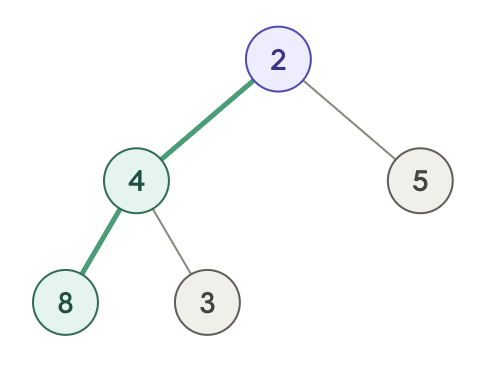
\includegraphics[width=0.5\textwidth]{../assets/Treemil.png}
\end{center}

\begin{lstlisting}
pub fn is_treemil(tree: Tree(Int)) -> Bool {
    // valid if:
    // 1. at least one child node is a multiple of its parent
    // 2. all children are valid treemils
    // leaves are valid treemils

    case tree {
        //is a leaf
        Tree(_, []) -> ________

        //is not a leaf
        Tree(label, branches) -> {
            let child_multiples = list.______(______, ______________)
            case list.________(child_multiples) >= 1 {
                True -> list.________(_____________________________)
                False -> ________
            }
        }
    }
}
\end{lstlisting}
\begin{questionmeta}
    This is a rewrite of the Tree recursion question treeil.
    We use a case statement which is basically an if statement, but you have to cover every case of the object you're referencing.
    \lstinline|Tree(_, [])| means a tree is a leaf: \lstinline|_| means that we don't care what's in the first element, and [] means that we're looking for a Tree where the branches list is empty.
\end{questionmeta}
\begin{solution}
\begin{lstlisting}
pub fn is_treemil(tree: Tree(Int)) -> Bool {
    case tree {
        Tree(_, []) -> True

        Tree(label, branches) -> {
            let child_multiples =
                list.filter(branches, fn(b) { b.label % label == 0 })
            case list.length(child_multiples) >= 1 {
                True -> list.all(list.map(branches, is_treemil), fn(x) { x })
                False -> False
            }
        }
    }
}
\end{lstlisting}
\end{solution}
\end{blocksection}

\begin{blocksection}
\question Implement \texttt{max\_treemil} which takes in a tree \texttt{t} and
determines the highest number of nodes in a treemil that is a subtree of
\texttt{t}. You may assume \texttt{is\_treemil} is implemented correctly from the
previous question.
\newline

\begin{lstlisting}
pub fn max_treemil(tree: Tree(Int)) -> Int {
    //Given a tree (that is not necessarily a treemil), returns
    //the highest number of nodes in a treemil in the tree.

    case tree {
        //is a leaf
        Tree(_, []) -> ________

        //is not a leaf
        Tree(_, branches) -> {
            case _____________________________ {
                True -> 1 + int.________(_____________________________)
                False -> result.unwrap(list.max(________, int.compare), 0)
            }
        }
    }
}
\end{lstlisting}
\begin{solution}
\begin{lstlisting}
pub fn max_treemil(tree: Tree(Int)) -> Int {
    case tree {
        Tree(_, []) -> 1

        Tree(_, branches) -> {
            case is_treemil(tree) {
                True -> 1 + int.sum(list.map(branches, max_treemil))
                False -> {
                    let sizes = list.map(branches, max_treemil)
                    result.unwrap(list.max(sizes, int.compare), 0)
                }
            }
        }
    }
}
\end{lstlisting}
\end{solution}
\begin{questionmeta}
    We had to do int.sum instead of just sum because this is the way Gleam works
    We had to do result.unwrap because the list.max function doesn't return a number, it returns a Result(Ok) or Result(Error), in case the max function was called on an empty list (in which case it would Error). We know that we're not calling it on an empty list, but the function doesn't know that.
    Result.unwrap says "I want to use the value from this list.max function if it was a valid result, and if the function errored we'll use the number in the second argument", which we put as 0. This means, we're using the max of the branches, and if the branches list was empty for some reason we'll use zero instead.
\end{questionmeta}
\end{blocksection}
